\documentclass[a4paper]{article}
%\pgfplotsset{compat=1.12}
%\usepackage{conference}
\usepackage{latexsym}
\usepackage[utf8x]{inputenc}
\usepackage[english]{babel}
\usepackage{amssymb,amsfonts,amsmath}
\usepackage{xcolor}
\usepackage{tikz}
\usepackage{tikz-3dplot}
\usepackage{pgfplots}
\usepackage{pgfplotstable}
\usepackage{cite}
\usepackage{hyperref}
\usepackage[varg]{txfonts}
\usepackage[T1]{fontenc}                   % Font encoding
\usepackage{geometry}
 \geometry{
 a4paper,
 total={170mm,257mm},
 left=20mm,
 top=20mm,
 }
%%%%%%
%%%%%%
\usetikzlibrary{patterns,arrows.meta,shapes,calc,angles,positioning,intersections,through,quotes,decorations.markings}
%\tdplotsetmaincoords{70}{110}
\usepackage{tkz-euclide}
\usetkzobj{all}
%%%%%%%
\def\doubleunderline#1{\underline{\underline{#1}}}
%%%%%%%
%%%%%%%

%% Begin of Watermark feature
%\usepackage[printwatermark]{xwatermark}
%\usepackage{xcolor}
%\newwatermark[allpages,color=red!50,angle=60,scale=6,xpos=0,ypos=0]{DRAFT}
%\newwatermark[allpages,color=red!20,angle=60,scale=2,xpos=0,ypos=0]{For Peer Review}
%% End of Watermark feature

\begin{document}

\title{Topological Axis in Macro and Micro \emph{physics}}

%\maketitle

%\begin{abstract}
%  The \emph{Topological Axis} is a convenient way of identifying large number correlations in Macro and Micro Physics domains.
%\end{abstract}

\begin{figure}
%\label{tab:9:table9}
\centering
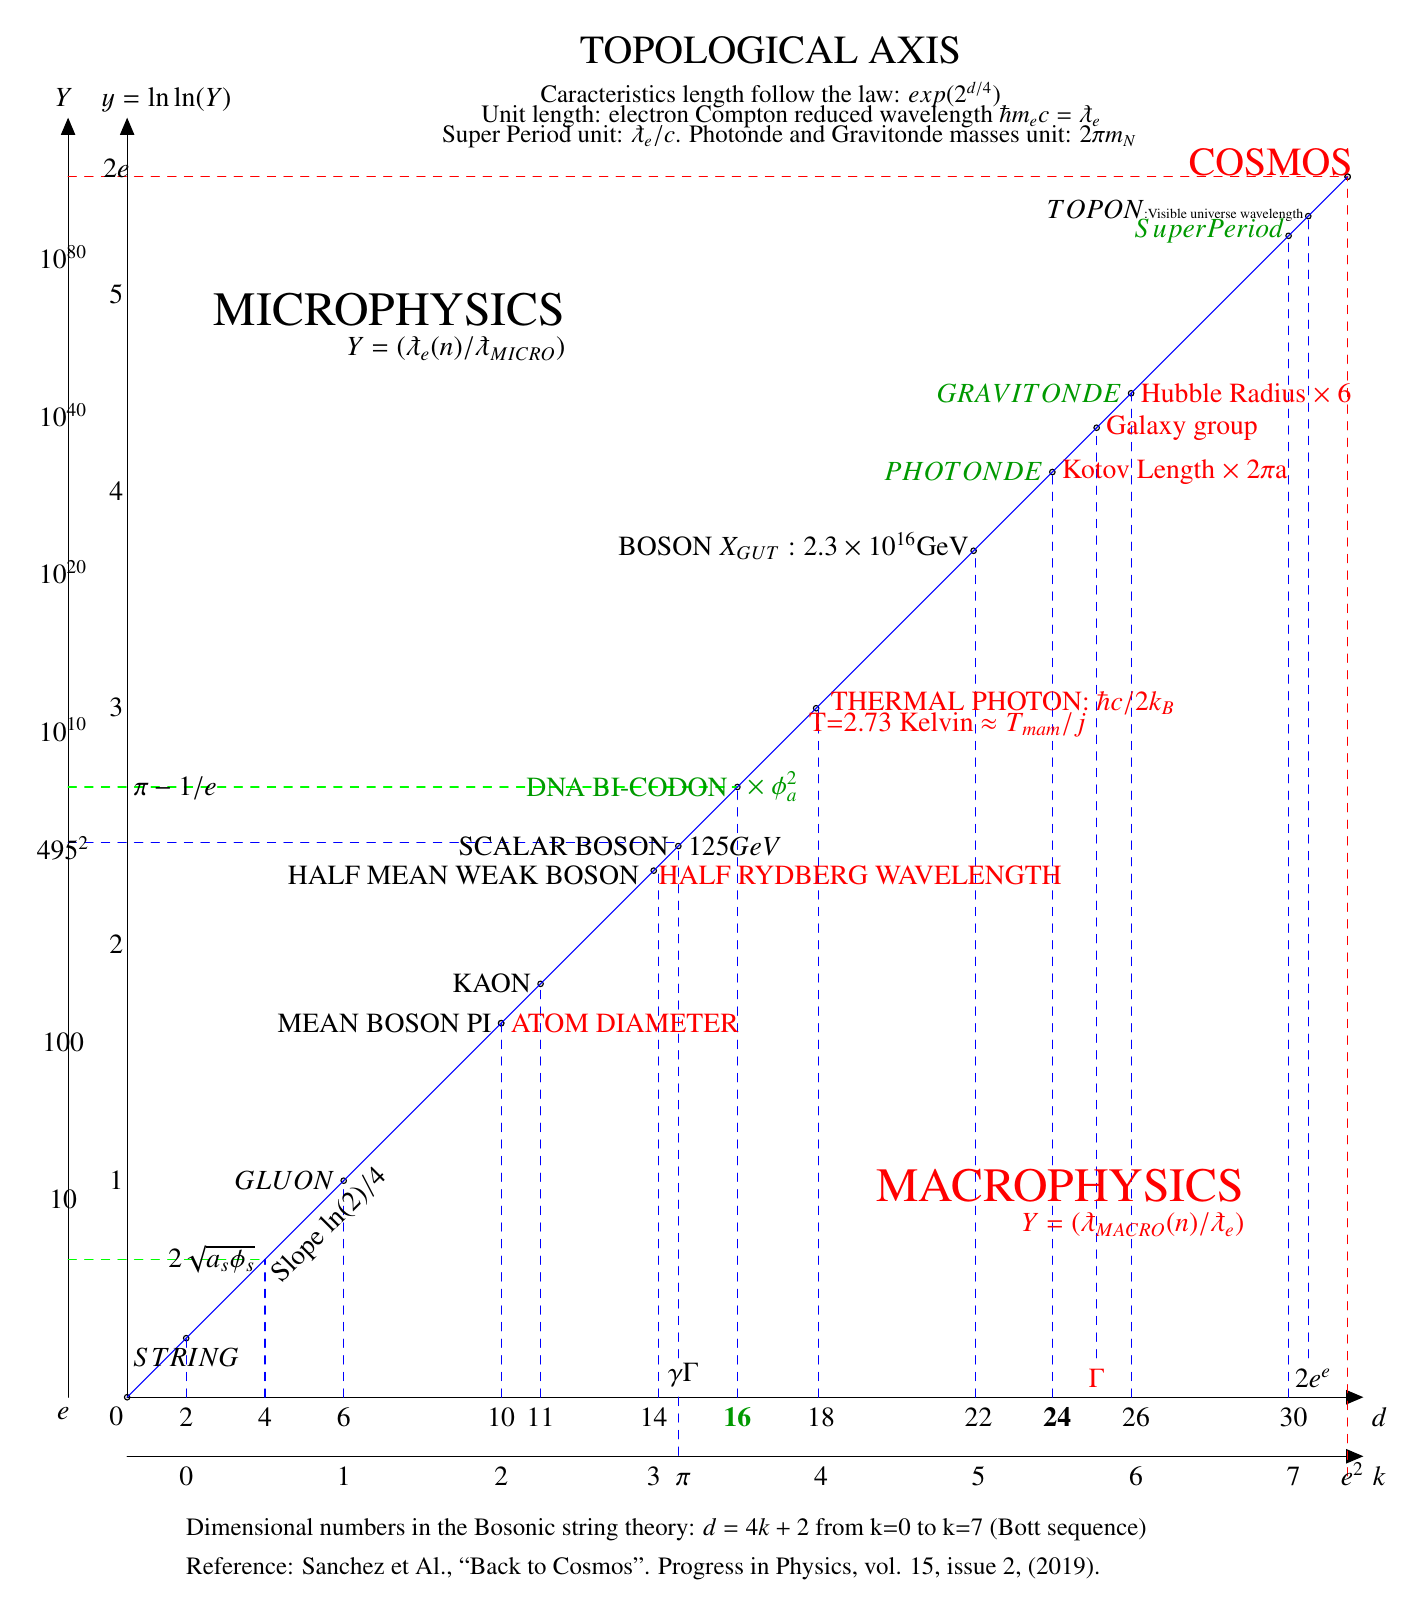
\begin{tikzpicture}[line cap=round,line join=round,>=triangle 
45,x=0.25cm,y=0.25cm]
%\begin{axis}[%
%width=\figurewidth,
%height=\figureheight,
%scale only axis,
%xmin=1,
%xmax=20,
%ymin=0,
%ymax=2,
%title={caracteristics length follow the law $exp(2^{d/4})$, unit length: electron compton reduced wavelength: $\hbar m_ec=\lambdabar_e$}, 
%legend style={draw=black,fill=white,legend cell align=left}
%]
%\draw[step=1cm,gray,very thin] (-31,-31) grid (31,31);
\tkzDefPoint(-31.0,-31.0){A} %\tkzDefPoint(5.,3.43){B} \tkzDefPoint(5.,0.){C} \tkzDefPoint(31.0,31.0){Y}
\tkzDefPoint(-28.0,-28.0){B}
\tkzDefPoint(-20.0,-20.0){C}
\tkzDefPoint(-12.0,-12.0){D}
\tkzDefPoint(-12.0,-12.0){E}
\tkzDefPoint(28.0,28.0){F}
\tkzDefPoint(-4.25,-4.25){G}
\tkzDefPoint(4.0,4.0){H}
\tkzDefPoint(12.0,12.0){I}
\tkzDefPoint(-3.0,-3.0){J}
\tkzDefPoint(16.0,16.0){K}
\tkzDefPoint(18.25,18.25){L}
\tkzDefPoint(20.0,20.0){M}
\tkzDefPoint(29.0,29.0){N}
\tkzDefPoint(-10.0,-10.0){P}
\tkzDefPoint[color=red](31.0,31.0){Q}
\tkzDefPoint(31.0,31.0){Y}
\tkzDrawPoints(A,B,C,D,F,E,G,H,I,J,K,L,M,N,P,Q,Y)
%\tkzMarkRightAngle(A,D,C)
%\tkzLabelPoints[text=red,right](G,H)
%\tkzMarkAngle[fill=blue!40,size=1.4cm,opacity=.5](C,A,B)
%\tkzLabelAngle[pos=1.6](C,A,B){$\theta$}
\tkzDefMidPoint(A,Y) \tkzGetPoint{BICODON}
\coordinate (center) at (BICODON);
%\tkzLabelPoints[below,color=green](BICODON)
\tkzDrawPoints(BICODON)
\draw [->] (-31.0,-31.0) node[left]{} -- (-31.,34.) node[right]{}; % scale Y
%\draw [->] (31.0,-31.0) node[left]{} -- (31.,31.) node[right]{}; % 
\draw [->] (-31.0,-31.0) node[left]{} -- (31.8,-31.0) node[right]{}; % scale d
\draw [->] (-31.0,-34.) node[left]{} -- (31.8,-34.) node[right]{};   % scale k
\draw [->] (-34.0,-31.) node[left]{} -- (-34.,34.) node[right]{};   % scale Y'
%%% Blue Dashed Horizontal lines
\draw [-,color=green,dashed] (-34.0,-24.) node[left]{} -- (-24.,-24.) node[right]{};   % \sqrt{a_s} horizontal line
\draw [-,color=blue,dashed] (-34.0,-2.8) node[left]{} -- (-2.8,-2.8) node[right]{};   % Scalar Boson horizontal line
\draw [-,color=green,dashed] (-34.0,0.) node[left]{} -- (0.,0.) node[right]{};   % bicodon horizontal line
\draw [-,color=red,dashed] (-34.0,31.) node[left]{} -- (31.,31.) node[right]{};   % Cosmos horizontal line
%%% Blue Dashed Vertical lines
\draw [-,color=blue,dashed] (-28.0,-31.) node[left]{} -- (-28.,-28.) node[right]{};   % String vertical line
\draw [-,color=blue,dashed] (-24.0,-31.) node[left]{} -- (-24.,-24.) node[right]{};   % \sqrt{a_s} vertical line
\draw [-,color=blue,dashed] (-20.0,-31.) node[left]{} -- (-20.,-20.) node[right]{};   % Gluon vertical line
\draw [-,color=blue,dashed] (-12.0,-31.) node[left]{} -- (-12.,-12.) node[right]{};   % ATOM DIAMETER vertical line
\draw [-,color=blue,dashed] (-10.0,-31.) node[left]{} -- (-10.,-10.) node[right]{};   % Kaon vertical line
\draw [-,color=blue,dashed] (-4.0,-31.) node[left]{} -- (-4.,-4.) node[right]{};   % Half Mean Weak Boson vertical line
\draw [-,color=blue,dashed] (-3.0,-29.) node[left]{} -- (-3.,-3.) node[right]{};   % Scalar Boson vertical line
\draw [-,color=blue,dashed] (-3.0,-31.) node[left]{} -- (-3.,-34.) node[right]{};   % \gamma\Gamma->\pi vertical line
\draw [-,color=blue,dashed] (0.,-31.) node[left]{} -- (0.,0.) node[right]{};   % Bicodon vertical line
\draw [-,color=blue,dashed] (4.1,-31.) node[left]{} -- (4.1,4.1) node[right]{};   % Thermal Photon vertical line
\draw [-,color=blue,dashed] (12.1,-31.) node[left]{} -- (12.1,12.1) node[right]{};   % Boson X GUT vertical line
\draw [-,color=blue,dashed] (16.,-31.) node[left]{} -- (16.,16.) node[right]{};   % Photon vertical line
\draw [-,color=blue,dashed] (18.25,-29.) node[left]{} -- (18.25,18.25) node[right]{};   % Galaxy group vertical line
\draw [-,color=blue,dashed] (20.0,-31.) node[left]{} -- (20.0,20.) node[right]{};   % Gravitonde vertical line
\draw [-,color=blue,dashed] (28.0,-31.) node[left]{} -- (28.0,28.0) node[right]{};   % Super Period vertical line
\draw [-,color=blue,dashed] (29.,-29.) node[left]{} -- (29.,29.0) node[right]{};   % Topon vertical line
\draw [-,color=red,dashed] (31.0,-35.) node[left]{} -- (31.,31.) node[right]{};   % Cosmos vertical line
%\draw[blue, dotted]
%      let \p1 =  ($(B)-(center)$),
%          \n0 = {veclen(\x1,\y1)}
%      in (center) circle(\n0);
%\draw[color=red] (-1.42,0.) -- (5.,0.);
%\draw[color=red] (5.,0.) -- (5.,3.43);
%\draw[color=red] (-1.42,0.) -- (5.,3.43);
\draw[color=blue] (A) -- (Y);
\node [anchor = text=blue] at (-8.,36.75) {\Large{TOPOLOGICAL AXIS}};
\node [anchor = text=black] at (-10.,34.75) {\small{Caracteristics length follow the law: $exp(2^{d/4})$}};
\node [anchor = text=black] at (-13.,33.75) {\small{Unit length: electron Compton reduced wavelength $\hbar m_e c=\lambdabar_e$}};
\node [anchor = text=black] at (-15.,32.75) {\small{Super Period unit: $\lambdabar_e/c$. Photonde and Gravitonde masses unit: $2\pi m_N$}};
\node [anchor = text=black] at (-28.,-38.0) {\small{Dimensional numbers in the Bosonic string theory: $d=4k+2$ from k=0 to k=7 (Bott sequence)}};
\node [anchor = text=black] at (-28.,-40.0) {\small{Reference: Sanchez et Al., ``Back to Cosmos''. Progress in Physics, vol. 15, issue 2, (2019).}};
\node [anchor = east,text=red] at (31.75,31.75) {\Large{COSMOS}};
\node [anchor = south] at (-28.,-33.0) {$2$};
\node [anchor = south] at (-28.,-36.0) {$0$};
\node [anchor = north] at (-28.,-28.0) {$STRING$};
\node [anchor = south] at (-24.,-33.0) {$4$};
\node [anchor = east] at (-24.,-24.0) {$2\sqrt{a_s\phi_s}$};
\node [anchor = south] at (-20.,-33.0) {$6$};
\node [anchor = south] at (-20.,-36.0) {$1$};
\node [anchor = east] at (-20.,-20.0) {$GLUON$};
\node [anchor = south] at (-12.,-33.0) {$10$};
\node [anchor = south] at (-10.,-33.0) {$11$};
\node [anchor = south] at (-12.,-36.0) {$2$};
\node [anchor = east] at (-12.,-12.) {MEAN BOSON PI};
\node [anchor = west,color=red] at (-12.,-12.) {ATOM DIAMETER};
\node [anchor = east] at (-10.,-10.) {KAON};
\node [anchor = south] at (-4.25,-33.0) {$14$};
\node [anchor = south] at (-4.25,-36.0) {$3$};
\node [anchor = east] at (-4.5,-4.5) {HALF MEAN WEAK BOSON};
\node [anchor = west,color=red] at (-4.5,-4.5){HALF RYDBERG WAVELENGTH};
\node [anchor = south] at (-2.75,-31.0) {$\gamma\Gamma$};
\node [anchor = south] at (-2.75,-36.0) {$\pi$};
\node [anchor = east,color=black] at (-3.0,-3.0){SCALAR BOSON};
\node [anchor = west,color=black] at (-3.0,-3.0){$125GeV$};
\node [anchor = south,color=black!40!green] at (0.,-33.0) {\textbf{16}};
\node [anchor = east,color=black!40!green] at (0.,0.0) {DNA BI-CODON};
\node [anchor = west,color=black!40!green] at (0.,0.0) {$\times$ $\phi_a^2$};
\node [anchor = south] at (4.25,-33.0) {$18$};
\node [anchor = south] at (4.25,-36.0) {$4$};
\node [cross,anchor = west,color=red] at (4.25,4.25){THERMAL PHOTON: $\hbar c/2k_B$};
\node [cross,anchor = west,color=red] at (3.15,3.15){T=2.73 Kelvin $\approx T_{mam}/j$};
\node [anchor = south] at (12.25,-33.0) {$22$};
\node [anchor = south] at (12.25,-36.0) {$5$};
\node [anchor = east,color=black] at (12.25,12.250){BOSON $X_{GUT}:2.3 \times 10^{16}$GeV};
\node [anchor = east,color=black!40!green] at (16.,16.){$PHOTONDE$};
\node [anchor = west,color=red] at (16.,16.){Kotov Length $\times$ $2\pi$a};
\node [anchor = west,color=red] at (18.25,18.250){Galaxy group};
\node [anchor = south,color=red] at (18.25,-31.0) {$\Gamma$};
\node [anchor = east,color=black!40!green] at (20.,20.0){$GRAVITONDE$};
\node [anchor = west,color=red] at (20.,20.0){Hubble Radius $\times$ 6};
\node [anchor = south] at (16.25,-33.0) {\textbf{24}};
\node [anchor = east,color=black!40!green] at (28.25,28.250){$Super Period$};
\node [anchor = east,color=black] at (29.25,29.250){$TOPON$\tiny{:Visible universe wavelength}};
\node [anchor = east,color=black] at (-8.25,24.250){\LARGE{MICROPHYSICS}};
\node [anchor = east,color=black] at (-8.25,22.250){$Y=(\lambdabar_e(n)/\lambdabar_{MICRO})$};
\node [anchor = east,color=red] at (26.25,-20.250){\LARGE{MACROPHYSICS}};
\node [anchor = east,color=red] at (26.25,-22.250){$Y=(\lambdabar_{MACRO}(n)/\lambdabar_{e})$};
\node [anchor = south] at (20.25,-33.0) {$26$};
\node [anchor = south] at (20.25,-36.0) {$6$};
\node [anchor = south] at (28.25,-33.0) {$30$};
\node [anchor = south] at (28.25,-36.0) {$7$};
\node [anchor = south] at (31.25,-36.0) {$e^2$};
\node [anchor = south] at (29.25,-31.0) {$2e^e$};
\node [anchor = south] at (32.6,-33.00) {$d$};
\node [anchor = south] at (32.6,-36.00) {$k$};
%%% Y AXIS
\node [anchor = north] at (-31.55,-31.0) {$0$};
\node [anchor = north] at (-31.55,-19.0) {$1$};
\node [anchor = north] at (-31.55,-7.0) {$2$};
\node [anchor = north] at (-31.55, 5.0) {$3$};
\node [anchor = north] at (-28.55, 1.0) {$\pi-1/e$};
\node [anchor = north] at (-31.55, 16.0) {$4$};
\node [anchor = north] at (-31.55, 26.0) {$5$};
\node [anchor = north] at (-31.55, 32.4) {$2e$};
\node [anchor = north] at (-29.0,36.0) {$y=\ln\ln(Y)$};
%%% Y' AXIS
\node [anchor = north] at (-34.25,-31.0) {$e$};
\node [anchor = north] at (-34.25,-20.0) {$10$};
\node [anchor = north] at (-34.25,-12.0) {$100$};
\node [anchor = north] at (-34.25,-2.0) {$495^2$};
\node [anchor = north] at (-34.25,4.0) {$10^{10}$};
\node [anchor = north] at (-34.25,12.0) {$10^{20}$};
\node [anchor = north] at (-34.25,20.0) {$10^{40}$};
\node [anchor = north] at (-34.25,28.0) {$10^{80}$};
\node [anchor = north] at (-34.25,36.0) {$Y$};
%% SLOPE
\tkzLabelSegment[sloped,below,text=black](A,D){Slope $\ln(2)/4$}
\end{tikzpicture}
%\caption[Topological Axis]{The Topological Axis follows the law $exp(2^{d/4})$ for its caracteristics lengths; its unit length: the electron compton reduced wavelength: $\hbar m_ec=\lambdabar_e$. it is the extrapolation toward smaller numbers of the Eddington's Double Larger Number correlation. The double natural logarithms y = ln(ln(Y)) of the main dimensionless physical quantities (Y) corresponds to the special string dimension series d = 4k + 2, from k = 0 to k = 7, characteristics of a Bott octonion sequence. This is the reunion of height 2D-1D holographic relations, hence the name `Topological Axis`.}
\end{figure}

%\bibliographystyle{unsrt}  
%\begin{thebibliography}{99}
%\bibitem{Sanchez} F.M. Sanchez, V. Kotov, M. Grosmann, D. Weigel, R. Veysseyre, C. Bizouard, N. Flawisky, D. Gayral, L. Gueroult, ``Back to Cosmos''. Progress in Physics, vol. 15, issue 2, (2019). http://www.ptep-online.com/2019/PP-57-12.PDF .\\
%\end{thebibliography}

\end{document}
